% Created 2023-03-01 Wed 09:36
% Intended LaTeX compiler: pdflatex
\documentclass[presentation,aspectratio=169]{beamer}
\usepackage[utf8]{inputenc}
\usepackage[T1]{fontenc}
\usepackage{graphicx}
\usepackage{grffile}
\usepackage{longtable}
\usepackage{wrapfig}
\usepackage{rotating}
\usepackage[normalem]{ulem}
\usepackage{amsmath}
\usepackage{textcomp}
\usepackage{amssymb}
\usepackage{capt-of}
\usepackage{hyperref}
\usepackage{khpreamble, euscript}
\DeclareMathOperator{\atantwo}{atan2}
\newcommand*{\ctrb}{\EuScript{C}}
\newcommand*{\obsv}{\EuScript{O}}
\usetheme{default}
\author{Kjartan Halvorsen}
\date{\today}
\title{El modelo canónico de robots móviles no-holonómicos}
\hypersetup{
 pdfauthor={Kjartan Halvorsen},
 pdftitle={El modelo canónico de robots móviles no-holonómicos},
 pdfkeywords={},
 pdfsubject={},
 pdfcreator={Emacs 26.3 (Org mode 9.4.6)}, 
 pdflang={English}}
\begin{document}

\maketitle

\section{Mobile robots}
\label{sec:org22ae9bb}

\section{Repetiión}
\label{sec:org33436d3}

\begin{frame}[label={sec:org9a790ed}]{De robot diferencial a modelo canónico}
\begin{columns}
\begin{column}{0.4\columnwidth}
\begin{center}
 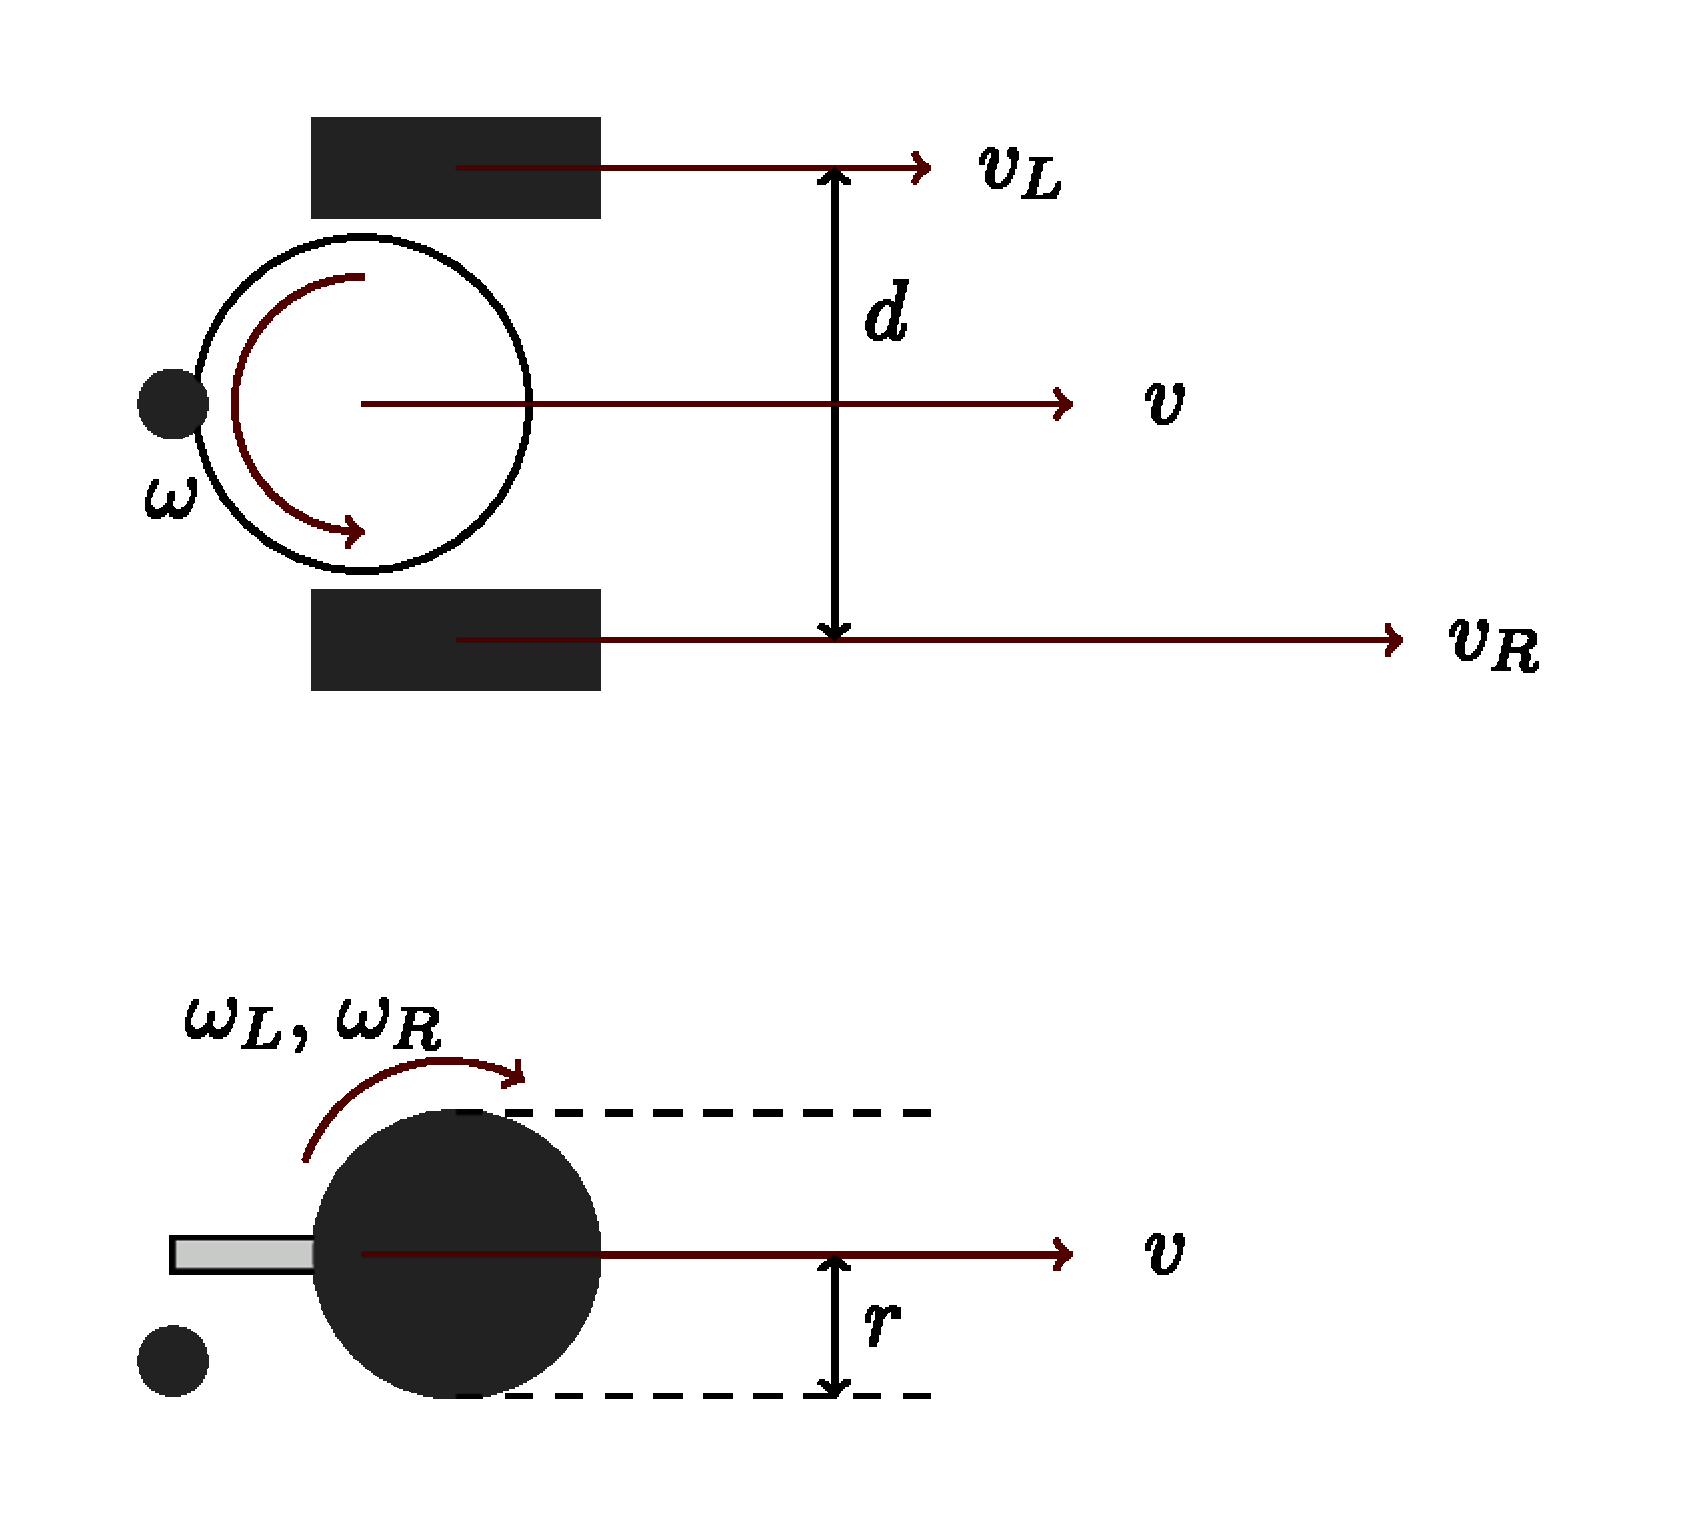
\includegraphics[width=1.0\linewidth]{../figures/unicycle-model-details}
\end{center}
\end{column}

\begin{column}{0.6\columnwidth}
\pause

\alert{Actividad} Encuentra las relaciones entre (\(\omega,\, v\)) y (\(\omega_L, \,\omega_R\))

\pause

\begin{align*}
  v &= \frac{v_L + v_R}{2} = \frac{r}{2} \big(\omega_L + \omega_L\big)\\
  \omega &= \frac{v_R - v_L}{d} = \frac{r}{d} \big(\omega_R - \omega_L\big)
\end{align*}

\begin{align*}
  \omega_L &= \frac{v_L}{r} = \frac{1}{r} \big(v - \frac{d}{2} \omega\big)\\
  \omega_R &= \frac{v_R}{r} = \frac{1}{r} \big(v + \frac{d}{2} \omega\big)
 \end{align*}
\end{column}
\end{columns}
\end{frame}

\begin{frame}[label={sec:org76e4d08}]{Diferencial a modelo canónico}
\begin{columns}
\begin{column}{0.4\columnwidth}
\begin{center}
 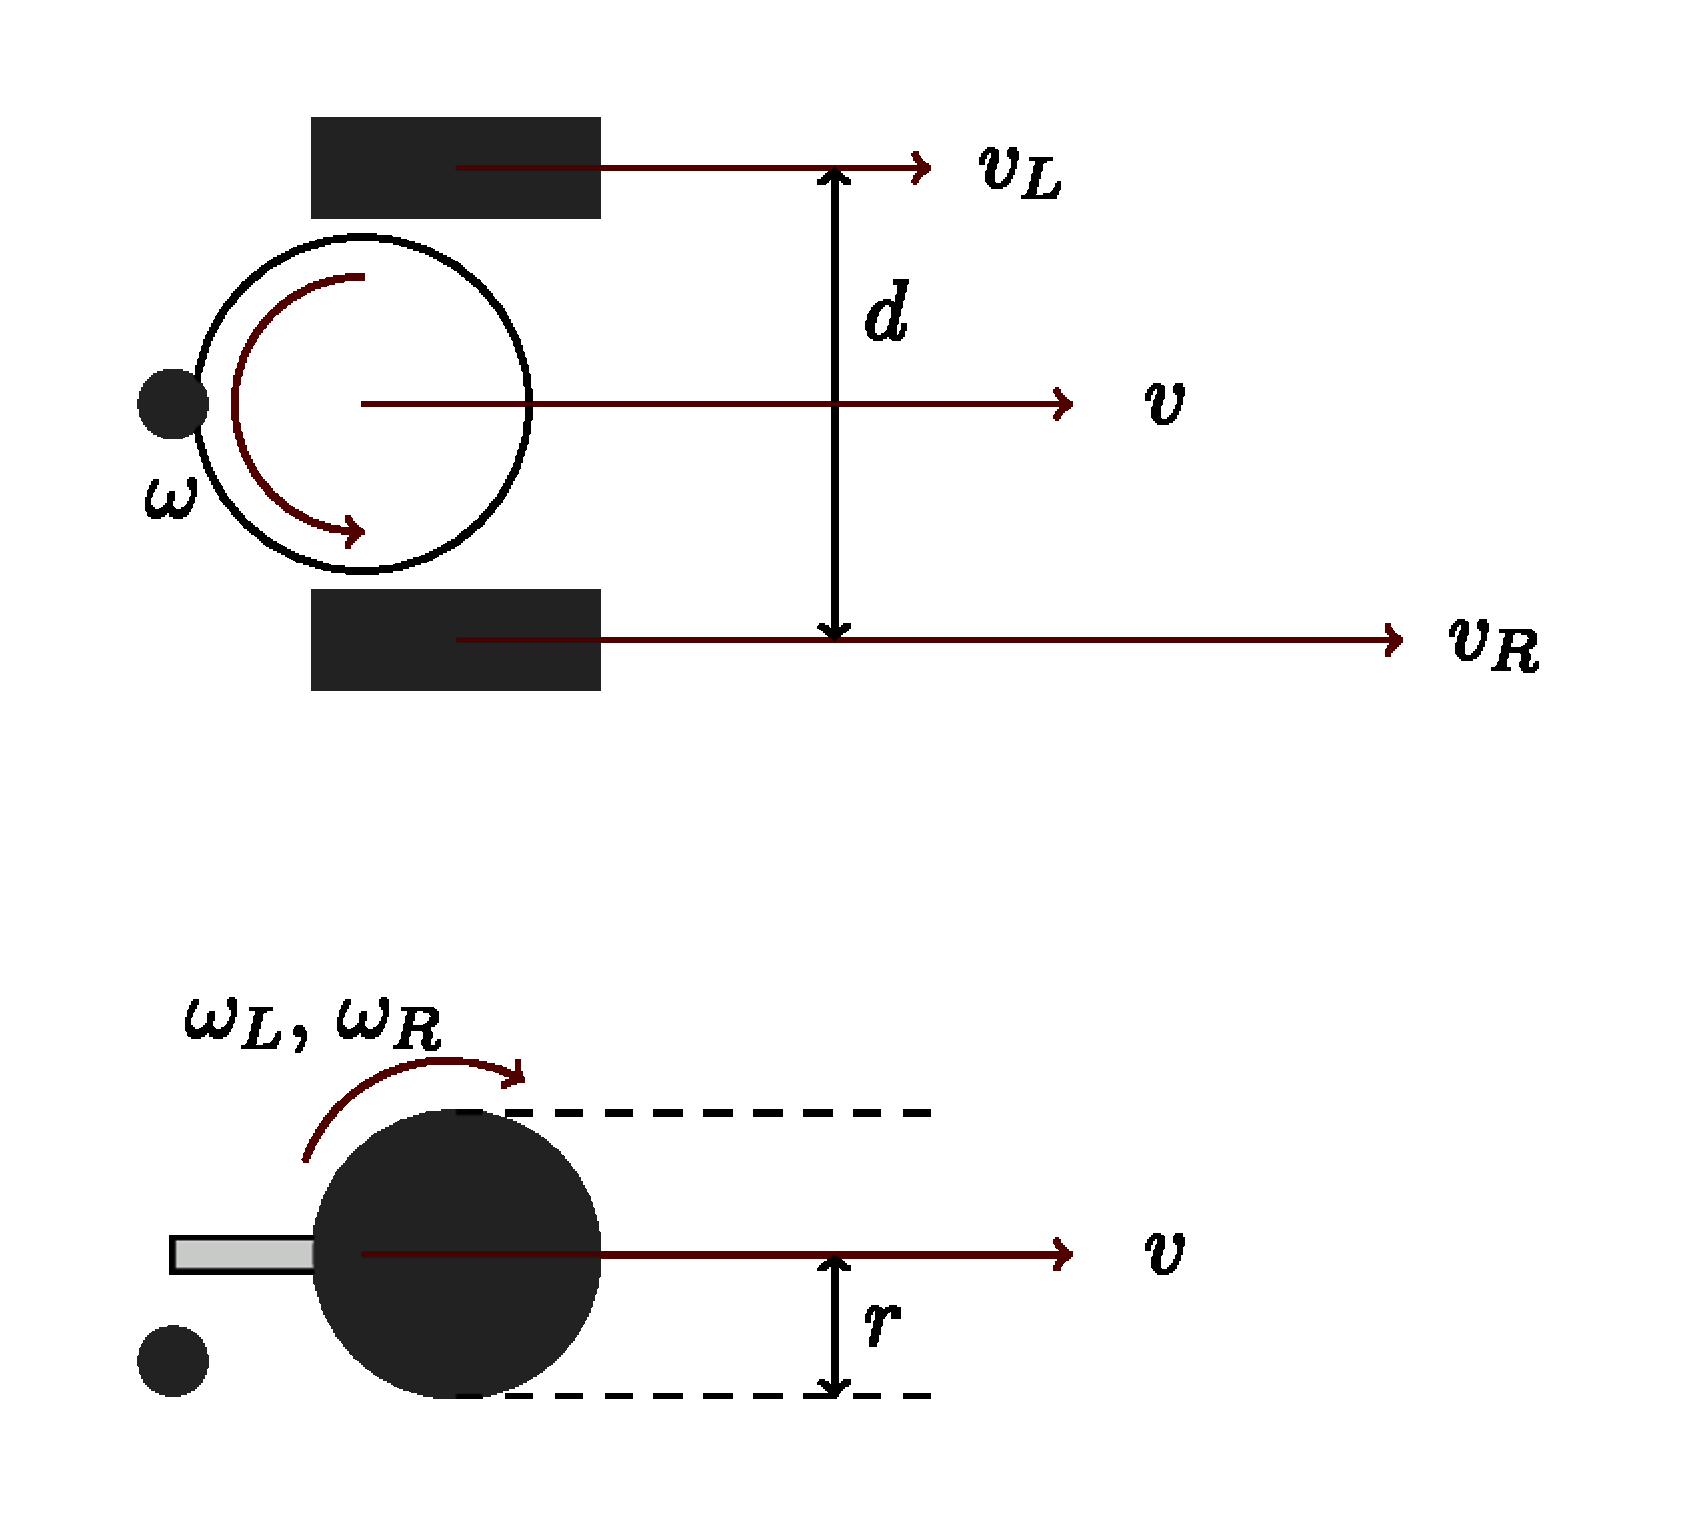
\includegraphics[width=.8\linewidth]{../figures/unicycle-model-details}
\end{center}
\end{column}

\begin{column}{0.6\columnwidth}
Asumiendo simetría entre las dos ruedas y en la dirección de giro.

\[ \omega_L,\, \omega_R \; \in \; [-\omega_{max}, \omega_{max}]\]

\pause

\alert{Actividad}
En el plano \(v,\, \omega\),  dibuje la región de posibles valores de la señal de entrada al modelo canónico,
\[ u(t) = \begin{bmatrix} \omega(t)\\v(t) \end{bmatrix}, \]
dado los límites de la velocidad angular de las ruedas.
\end{column}
\end{columns}
\end{frame}

\begin{frame}[label={sec:orgb1fb872}]{Diferencial a modelo canónico}
\begin{columns}
\begin{column}{0.4\columnwidth}
\begin{center}
 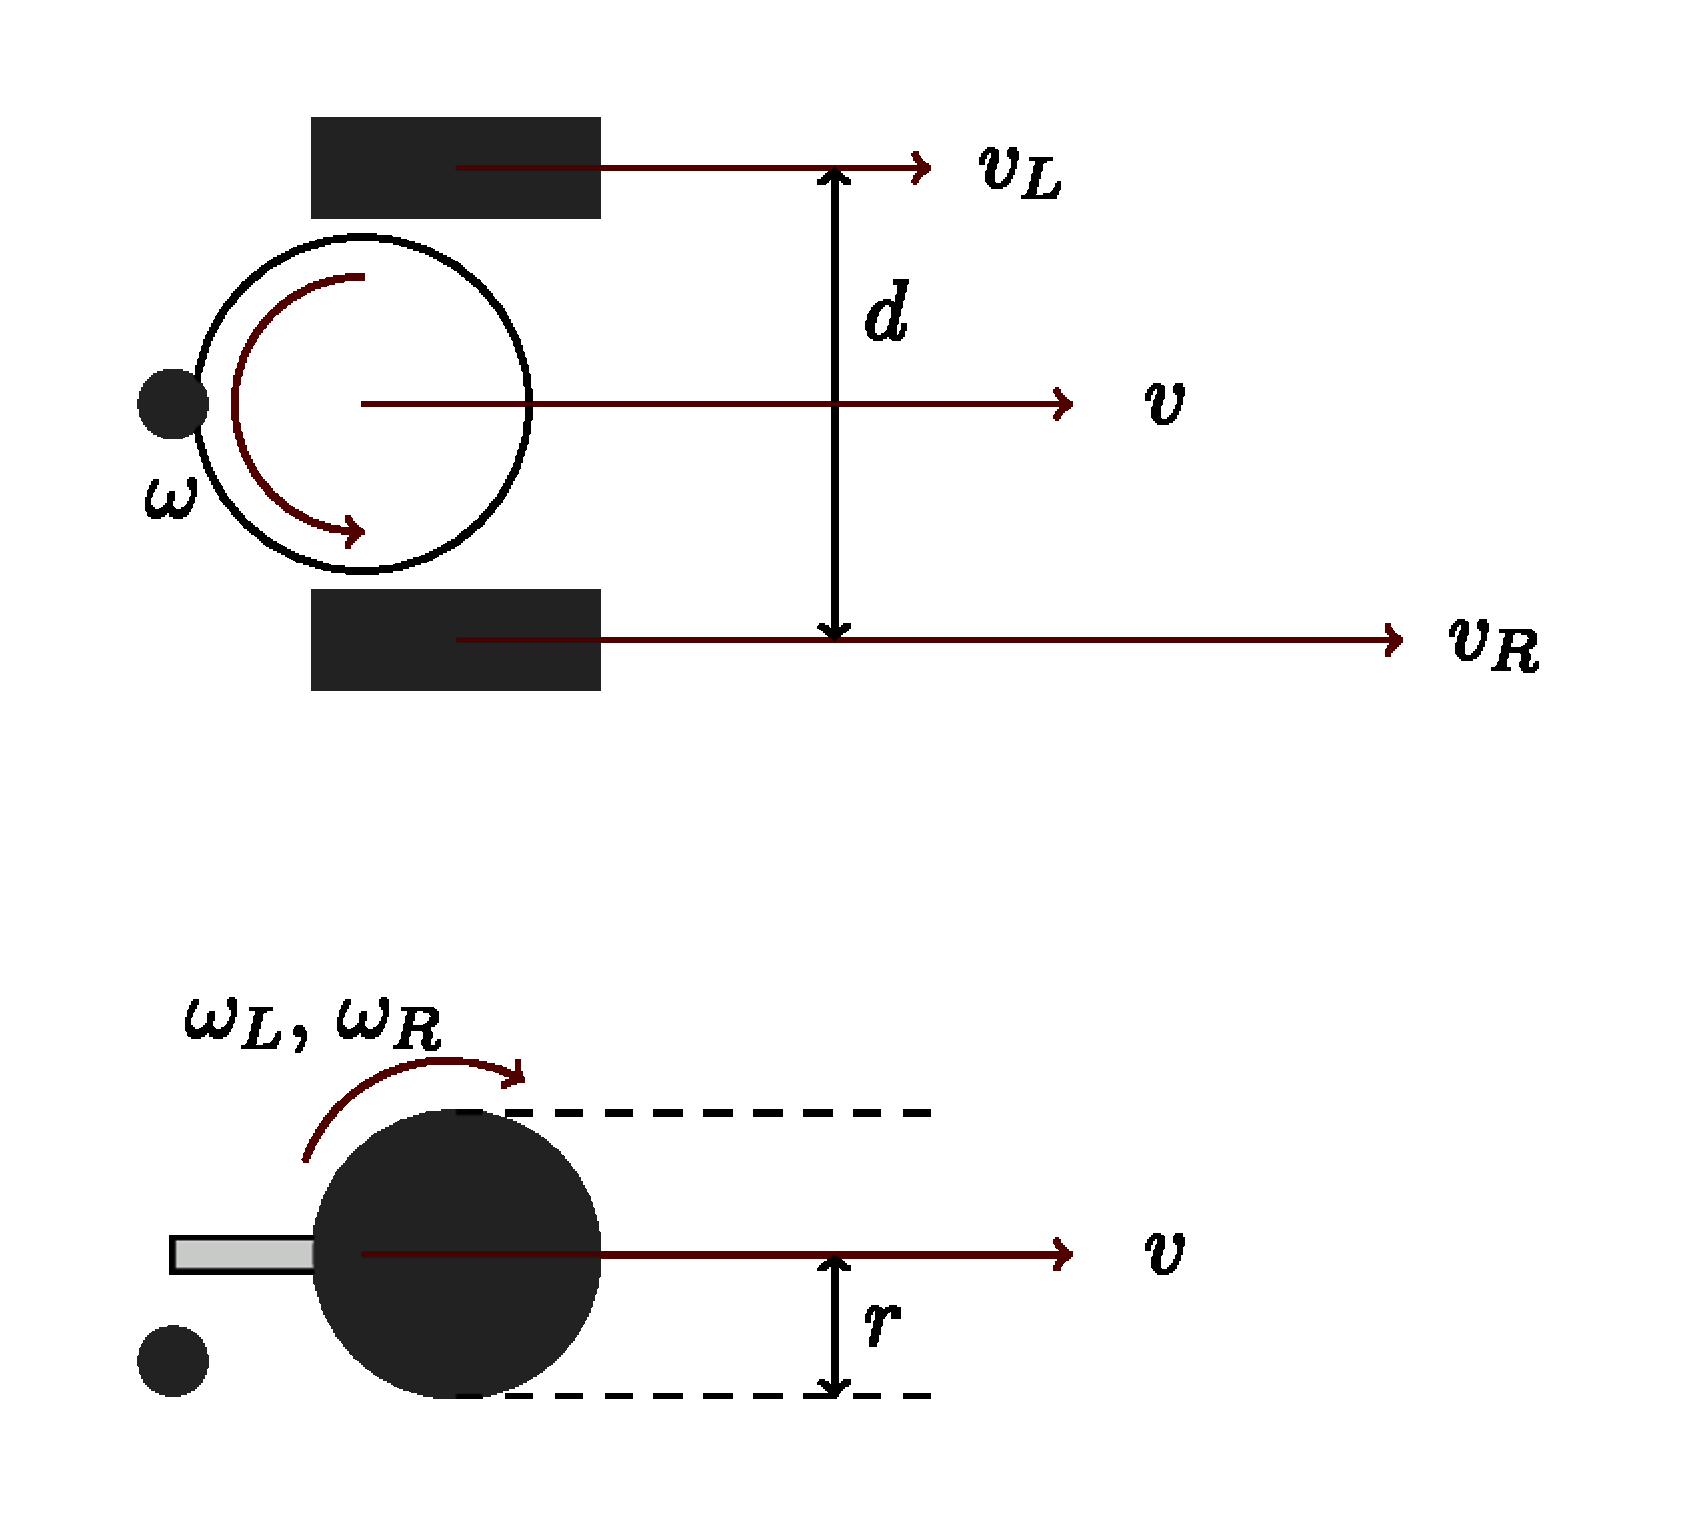
\includegraphics[width=.8\linewidth]{../figures/unicycle-model-details}
\end{center}
\end{column}

\begin{column}{0.6\columnwidth}
\begin{center}
  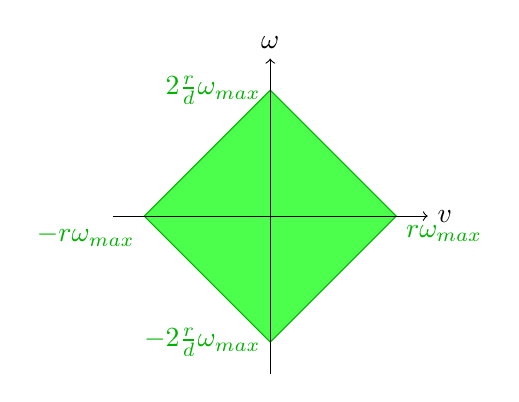
\begin{tikzpicture}[scale=1]
  \pgfmathsetmacro{\wwmax}{16}
  \pgfmathsetmacro{\dd}{2}
  \pgfmathsetmacro{\rr}{0.1}
  \pgfmathsetmacro{\vmax}{\rr * \wwmax}
  \pgfmathsetmacro{\wmax}{2*\wwmax * \rr / \dd}
  
  \draw[green!70!black, fill=green!70]  (0, \wmax) node[left] {$2\frac{r}{d}\omega_{max}$}
  --  (\vmax, 0)
  node[below right] {$r\omega_{max}$} -- (0, -\wmax) node[left]{$-2\frac{r}{d}\omega_{max}$}
  --  (-\vmax, 0) node[below left] {$-r\omega_{max}$} -- (0, \wmax);
  
  \draw[->] (-2,0) -- (2, 0) node[right] {$v$};
  \draw[->] (0,-2) -- (0,2) node[above] {$\omega$};
\end{tikzpicture}
\end{center}
\end{column}
\end{columns}
\end{frame}


\section{Car-like}
\label{sec:org55d7b13}

\begin{frame}[label={sec:orgb0b4836}]{Robots tipo coche - modelo bicicleta}
\begin{columns}
\begin{column}{0.4\columnwidth}
\begin{center}
 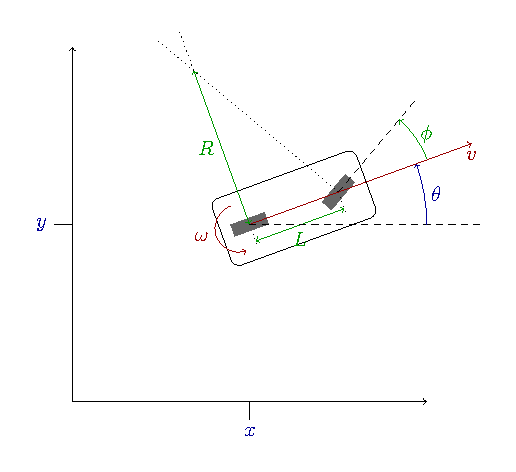
\includegraphics[width=1.05\linewidth]{../figures/bicycle-model}
\end{center}
\end{column}

\begin{column}{0.6\columnwidth}
\pause

Para un robot que se mueve instantaneamente en una trayectoria círcular con radie \(R\), la relación entre su velocidad lineal \(v\) y su velocidad angular \(\omega\) es

\pause

\[ v = R\omega \quad \Rightleftarrow \quad \omega = \frac{1}{R} v \]

\pause
\alert{Actividad} Determine el radie de giro instantaneo \(R\) como función del ángulo de dirección \(\phi\).

\pause
\alert{Actividad} Determine la velocidad angular \(\omega\) como función de la velocidad \(v\) y del ángulo de dirección \(\phi\). Determine también la función inversa.
\end{column}
\end{columns}
\end{frame}



\begin{frame}[label={sec:org7fbcf45}]{Robots tipo coche - modelo bicicleta}
\begin{columns}
\begin{column}{0.4\columnwidth}
\begin{center}
 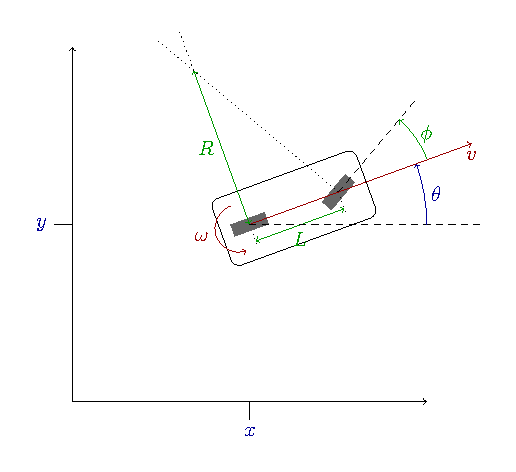
\includegraphics[width=1.05\linewidth]{../figures/bicycle-model}
\end{center}
\end{column}

\begin{column}{0.6\columnwidth}
Para cierto robot
\[ v \in [-v_{lm}, v_{um}], \quad \phi \in [-\phi_{max}, \phi_{max}]\]


\pause

\alert{Actividad} En el plano \(v,\, \omega\), dibuje la región de posibles valores de la señal de entrada al modelo canónico,
\[ u(t) = \begin{bmatrix} \omega(t)\\v(t) \end{bmatrix}, \]
dado los límites de la velocidad \(v\) y del ángulo de dirección \(\phi\).
\end{column}
\end{columns}
\end{frame}
\end{document}